\documentclass[12pt]{article}

\usepackage{amsmath}
\usepackage{graphicx}
\usepackage[margin=1.1in]{geometry}
\usepackage{tcolorbox}



\title{Special Theory of Relativity and Field Transformations}
\author{İ. Yalçınkaya}
\date{\today}

\begin{document}

\maketitle

\section*{§1. The Notion of Event}
An \textit{event} is something that occurs at a specific point in space and time, such as the emission of a light pulse or the collision of two particles. It is specified by four parameters, conventionally written as a column vector:
\[
\mathbf{x} = \begin{pmatrix}
x\\
y\\
z\\
t
\end{pmatrix}
\]
where $x$, $y$, and $z$ are the spatial coordinates of the event, and $t$ is the time at which the event occurs. By convention these parameters are called the \textit{spacetime coordinates} of the event. These coordinates are defined within a given reference frame and describe where and when the event occurs, not when it is observed. Because signals propagate at the finite speed of light, observation generally involves a delay; this delay is not part of the event’s coordinates.

Operationally, one can imagine space filled with synchronized clocks at rest in the chosen frame. The time coordinate of an event is then the reading of the clock located at the event’s position when it occurs. This convention provides a consistent way to assign spacetime coordinates by overcoming the issue of signal propagation delay.

\section*{§2. Galilean Transformations}

An event can be described by different observers. If two observers are in relative motion, they generally assign different coordinates to the same event. Consider two inertial frames $S$ and $S'$ where $S'$ moves with constant velocity $V$ along the x-axis of $S$ as shown in Figure \ref{fig:1}. The axes are chosen so that the x-axes coincide with the direction of motion, while the y and z axes are parallel. Event $E$ which is described by coordinates $(x,y,z,t)$ in frame $S$ is described by coordinates $(x',y',z',t')$ in frame $S'$. The transformation between these coordinates as

\begin{figure}[h]
\centering
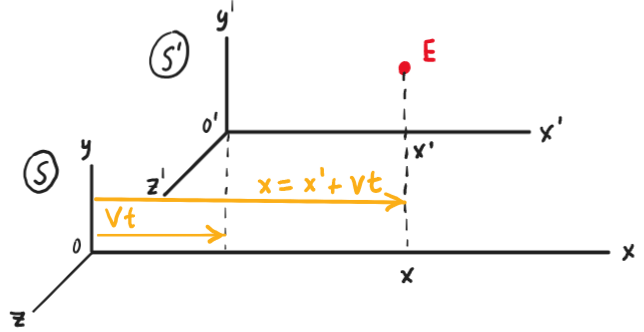
\includegraphics[width=0.6\textwidth]{fig1.png}
\caption{Inertial frames $S$ and $S'$ moving relative to each other.}
\label{fig:1}
\end{figure}

\[
\begin{pmatrix}
x'\\
y'\\
z'\\
t'
\end{pmatrix}=
\begin{pmatrix}
x-Vt\\
y\\
z\\
t
\end{pmatrix}
\]
Equivalently, the same transformation can be written in matrix--vector form as
\[
\underbrace{\begin{pmatrix}
x'\\
y'\\
z'\\
t'
\end{pmatrix}}_{\mathbf{x'}}
=
\underbrace{\begin{pmatrix}
1 & 0 & 0 & -V\\
0 & 1 & 0 & 0\\
0 & 0 & 1 & 0\\
0 & 0 & 0 & 1
\end{pmatrix}}_{G}
\underbrace{\begin{pmatrix}
x\\
y\\
z\\
t
\end{pmatrix}}_{\mathbf{x}}
\]
where $G$ is the matrix representing the transformation. This transformation is called the \textit{Galilean transformation} and assumes that time is absolute and the same for all observers ($t' = t$). Once the coordinates of an event $\mathbf{x}$ are known in $S$ frame, the coordinates in $S'$ frame can be found by multiplying $\mathbf{x}$ by the matrix $G$, $\mathbf{x'} = G\mathbf{x}$. The inverse transformation can be obtained by replacing $V$ with $-V$ in the matrix $G$. Note that the transformation matrix $G$ depends on the relative velocity $V$ between the two frames.

If a particle's position in frame $S$ is given by the function $x(t)=vt$, where $v$ is the velocity of the particle in frame $S$, then its position in frame $S'$ is given by $$x'(t'=t) = x(t) - Vt = vt - Vt = (v-V)t.$$ Therefore, if $V<v$, the particle moves slower in $x$ direction in frame $S'$ than in frame $S$. If $V=v$, the particle is at rest in frame $S'$. If $V>v$, the particle moves faster in $-x$ direction in frame $S'$. This illustrates how the velocity of a particle transforms under Galilean transformations. This is known as the \textit{velocity addition formula} in classical mechanics, which states that the velocity of a particle in one frame is equal to its velocity in another frame plus the relative velocity between the two frames.

Obviously, the function $x(t)=vt$ is the equation of motion for the particle and it is not a single event. From this point of view, the equation of motion of a particle should be treated as a continuous set of consecutive events, each of which can be transformed using the Galilean transformation. 

\section*{§3. Lorentz Transformation}

Experiments (Michelson-Morley) have shown that the velocity addition formula of classical mechanics does not hold for light. The speed of light in vacuum is always measured to be the same, regardless of the motion of the source or observer. In other words, light cannot be chased or overtaken. It does not matter how fast the observers are moving with respect to each other; if a light ray is moving through vacuum at speed $c$, it will always be measured to have speed $c$ by any observer. Maxwell's equations are also consistent with a frame-independent speed of light. Therefore, the Galilean transformations must be modified to be consistent with the invariance of the speed of light.

From the mathematical point of view, we stop considering Galilean transformations as the only possible transformations between inertial frames, we can look for more general linear transformations that could relate the coordinates of an event in one frame to those in another frame. In other words, we are looking for a transformation matrix $L$ such that
\[\mathbf{x'} = L\mathbf{x}
\]and that satisfies the condition that the speed of light is invariant. By assuming that the axes of the two frames are parallel and that the relative motion is along the x-axis, and assuming that the space is \textit{isotropic} and \textit{homogeneous}, the most general transformation turns out to be a linear transformation of the form
\[
x' = Ax + Bt
\]
\[t' = Dx + Et
\]
where $A$, $B$, $D$, and $E$ are constants which will be determined soon. Thus, once we are given $x$ and $t$, we can find $x'$ and $t'$. First, note that we did not assume that $t' = t$ as in the Galilean transformation, so we are allowing for the possibility that time may not be absolute. Second, the reason that the structure of these transformations is linear can be directly followed from the homogenity and isotropy of space and time. Homogeneity of space and time means:
\begin{itemize}
\item There is no special point in space.
\item There is no special moment in time.
\end{itemize}
Mathematically, it equivalently means that the physics is invariant under translations:
\[(x,t)\rightarrow (x+a, t+b)\]
where $a$ and $b$ are arbitrary constants. Assume that the transformation is nonlinear, then we can write it as
\[
x' = f(x,t)
\]
where the function $f$ contains higher order terms of $x$ and $t$. Consider two events in $S$ separated by $(x_2-x_1, t_2-t_1)$. Homogeneity of space and time requires that the transformation of these two events should depend only on their separation, not on their absolute coordinates. Therefore,
\[x'_2-x'_1 = f(x_2,t_2) - f(x_1,t_1)\]
must depend only on $(x_2-x_1, t_2-t_1)$. The only function that satisfies this condition is a linear function, which can be written as
\[f(x,t) = Ax + Bt+C.\]
The constant $C$ only shifts the origin, so once the origins are aligned, we can set $C=0$:
\[x' = Ax + Bt.
\]

\begin{tcolorbox}[colback=yellow!20, colframe=black]
\textbf{Try:} Assume that the transformation is nonlinear $f(x,t)= Ax^2 + Bt^2$ and redo the above argument to show that this transformation does not satisfy the homogeneity condition.
\end{tcolorbox}

The isotropy of space means that there is no preferred direction in space. This implies that the transformation should be symmetric with respect to the direction of motion. Therefore, if we reverse the direction of motion (i.e., replace $V$ with $-V$), the form of the transformation should remain unchanged. 


Now let us determine the constants $A$, $B$, $D$, and $E$. First, consider the motion of the origin of $S'$ frame as observed in $S$ frame. Since the origin of $S'$ is moving with velocity $V$ along the x-axis of $S$, if an event occurs at the origin of $S'$ frame, its coordinates in $S$ frame will be $(x,t)=(Vt,t)$:
\[0=Ax + Bt = AVt + Bt\]
which implies that
\[B = -AV \rightarrow x' = A(x - Vt).
\]


Now let us enforce the invariance of the speed of light. Assume that a light pulse is emitted at the common origin of the two frames at time $t=t'=0$. In frame $S$, the coordinates of the event of light emission are $(x,t)=(0,0)$, and after a time $t$, the light pulse will have traveled a distance $ct$ from the origin (in the both $\pm x$ directions), so its coordinates will be $(\pm ct,t)$~\footnote{The light pulse actually propagates in all directions, but since there is no relative motion in $y$ and $z$ directions, we only consider the $x$-direction.}. In frame $S'$, the coordinates of the same event will be $(ct',t')$ since the speed of light is an invariant. If we plug these coordinates into the transformation equations, we get
\[x' = A(ct - Vt) = A(c-V)t\]
\[t' = D(ct) + Et = (Dc+E)t
\]
Imposing $x' = ct'$ gives us
\[A(c-V) = c(Dc + E)\]
Doing the same for $x=-ct$ gives
\[A(-c-V) = -c(-Dc + E)\]
Solving these two equations, we find that
\[
D=-\frac{AV}{c^2}~~ \text{and} ~~E=A.
\]
What we have found so far is that the transformation can be written as
\[x' = A(x - Vt)
\]
\[t' = A\left(t - \frac{V}{c^2}x\right)
\]

Now we need to determine the constant $A$. By the relativity principle, going from $S$ to $S'$ with velocity $V$ must have the same form as going back from $S'$ to $S$ with velocity $-V$. So, inverse must be 
\[x = A(x' + Vt')
\]
\[t = A\left(t' + \frac{V}{c^2}x'\right)
\]
Substituting the expressions for $x'$ and $t'$ into the above equations, we get
\[x = A^2\left(x - \frac{V^2}{c^2}x\right) = A^2\left(1 - \frac{V^2}{c^2}\right)x\]
\[t = A^2\left(t - \frac{V^2}{c^2}t\right) = A^2\left(1 - \frac{V^2}{c^2}\right)t   \]  
Above equations must hold for all $x$ and $t$, which implies that $A^2(1 - \frac{V^2}{c^2}) = 1$:
\[A = \frac{1}{\sqrt{1 - \frac{V^2}{c^2}}} \equiv \gamma
\]
where $\gamma$ is called the \textit{Lorentz factor}. We chose the positive root because at $V=0$, we have $A=1$. Therefore, the final form of the transformation is
\[x' = \gamma(x - Vt)
\]
\[t' = \gamma\left(t - \frac{V}{c^2}x\right)
\]
This transformation is called the \textit{Lorentz transformation}. It reduces to the Galilean transformation in the limit of low velocities ($V \ll c$) since $\gamma \approx 1$ in that limit. The Lorentz transformation shows that space and time are intertwined and that time is not absolute but depends on the relative motion of the observer. It also leads to many counterintuitive consequences such as time dilation and length contraction.

Equivalently, Lorentz transformations can be written in a matrix-vector product form as follows:

\[
\underbrace{\begin{pmatrix}
x'\\
y'\\
z'\\
t'
\end{pmatrix}}_{\mathbf{x'}}
=
\underbrace{\begin{pmatrix}
\gamma & 0 & 0 & -V\gamma\\
0 & 1 & 0 & 0\\
0 & 0 & 1 & 0\\
-\gamma V/c^2 & 0 & 0 & \gamma
\end{pmatrix}}_{L}
\underbrace{\begin{pmatrix}
x\\
y\\
z\\
t
\end{pmatrix}}_{\mathbf{x}}.
\]
Therefore, the transformation matrix now contains information about the relative speed of two reference frames and the speed of light. Note that this representation is not the conventional representation of Lorentz trasnformations, and the convenient form of this trasnformation will be given later.

\section*{§4. Relativity of Simultanity}
Events that are simultaneous in one frame are generally not simultaneous in another. Let us show this by using Lorentz transformations. Consider two events in $S$, $(x_1,t_1)$ and $(x_2,t_2)$, and suppose that they are simultaneous, $t_1=t_2$. Define the position and time difference in $S$ frame as $\Delta x \equiv x_2-x_1$ and $\Delta t \equiv t_2-t_1 = 0$, respectively. Then, Time and time intervals transform as 
\[
t' = \gamma \left( t - \frac{Vx}{c^2} \right) \rightarrow \Delta t' = \gamma \left( \Delta t - \frac{V\Delta x}{c^2} \right) =\gamma \left( \frac{V\Delta x}{c^2} \right) 
\]

\[
\Delta t' = \frac{\gamma V}{c^2}\Delta x \neq 0 
\]
This means that if two events happen at different places and are simultaneous in $S$, they are not simultaneous in $S'$.


\section*{§5. Time Dilation}

Let us consider to events, in particular, two ticks of a clock that is at rest in frame $S'$. The coordinates of these two events in $S'$ frame are $(x',t')=(0,0)$ and $(0, t')$, where $t'$ is the time interval between the two ticks as measured in $S'$. Since the clock is at rest in $S'$, its spatial coordinate does not change. A clock at rest in $S'$ moves in $S$, so: $x = Vt$. If we plug this into the time transformation equation, we get
\[t' = \gamma\left(t - \frac{V}{c^2}x\right) = \gamma\left(t - \frac{V^2}{c^2}t\right) = \gamma t\left(1 - \frac{V^2}{c^2}\right) = \frac{t}{\gamma}
\]
Therefore, if two ticks are seperated by $\Delta t'$ in frame $S'$, and by the same two ticks are seperated by $\Delta t$ in frame $S$, we have
\[\Delta t' = \frac{\Delta t}{\gamma} \rightarrow \Delta t = \gamma \Delta t'   
\]

\begin{figure}[h]
\centering
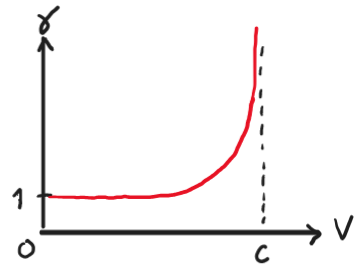
\includegraphics[width=0.35\textwidth]{fig2.png}
\caption{The Lorentz factor $\gamma$ as a function of velocity $V/c$.}
\label{fig:2}
\end{figure}

Since $\gamma > 1$ for $V > 0$ as shown in Figure 2, we have $\Delta t > \Delta t'$. This means that the time interval between two ticks of the clock is longer in frame $S$ than in frame $S'$. In other words, the clock runs slower in $S$ than in $S'$. This phenomenon is called \textit{time dilation}. It implies that moving clocks run slower compared to stationary clocks. The faster the relative velocity $V$, the greater the time dilation effect, and as $V$ approaches the speed of light $c$, the time dilation becomes more pronounced. The time interval $\Delta t'$ measured in the rest frame of the clock is called the \textit{proper time}, which means it is the time interval measured by an observer who is at rest relative to the clock, or in other words, it is interval measured by the clock itself.

\section*{§6. Length Contraction}
Length is the distance between two endpoints measured at the same time in a given frame. Let a pieace of rod be at rest in frame $S'$. So the endpoint are fixed in $S'$. The length of the rod which is defined in the rest frame $S'$ is called the \textit{proper length} and denoted by $L_0 \equiv \Delta x'$. If we want to measure the length of the rod in frame $S$, we need to measure the positions of the two endpoints at the same time in $S$. This is because the endpoints of the rod are moving in $S$, so if we measure them at different times, we would be measuring the position of one endpoint at a different time than the other endpoint, which would not give us the correct length of the rod in $S$. Therefore, the measurement events at the end points must be simultaneous in $S$ to get the correct length of the rod in $S$. Let us say that we measure the positions of the endpoints at time $t$ in $S$. The coordinates of the endpoints in $S'$ are given by
\[x' = \gamma(x - Vt)
\]
Since the endpoints are fixed in $S'$, we have $\Delta x' = \gamma(\Delta x - V\Delta t)$. But we measure the endpoints at the same time in $S$, so $\Delta t = 0$. Therefore, we have
\[\Delta x' = \gamma \Delta x \rightarrow \Delta x = \frac{\Delta x'}{\gamma} = \frac{L_0}{\gamma}
\]
Since $\gamma > 1$ for $V > 0$, we have $\Delta x < \Delta x'$. This means that the length of the rod is shorter in frame $S$ than in frame $S'$. This phenomenon is called \textit{length contraction}. It implies that moving objects are measured to be shorter along the direction of motion compared to their proper length. The faster the relative velocity $V$, the greater the length contraction effect, and as $V$ approaches the speed of light $c$, the length contraction becomes more pronounced. Length contraction only occurs along the direction of relative motion; there is no contraction in the directions perpendicular to the motion. 

\section*{§7. Relativistic Velocity Addition}
A particle is moving with velocity $u'=dx'/dt'$ in frame $S'$. The same particle's velocity is observed as $u=dx/dt$ in frame $S$. We can find the relationship between $u$ and $u'$ by differentiating the Lorentz transformation equations with respect to time $t$. From the spatial transformation, we have
\[\frac{dx'}{dt} = \gamma\left(\frac{dx}{dt} - V\right) = \gamma(u - V)
\]From the time transformation, we have
\[\frac{dt'}{dt} = \gamma\left(1 - \frac{V}{c^2}\frac{dx}{dt}\right) = \gamma\left(1 - \frac{Vu}{c^2}\right)
\]Therefore, the velocity of the particle in $S'$ frame is given by
\[u' = \frac{dx'}{dt'} = \frac{\gamma(u - V)}{\gamma\left(1 - \frac{Vu}{c^2}\right)} = \frac{u - V}{1 - \frac{Vu}{c^2}} \]
This is the \textit{relativistic velocity addition formula}. It shows how velocities transform between different inertial frames in special relativity. If we want to find the velocity of the particle in $S$ frame given its velocity in $S'$ frame, we can solve the above equation for $u$:
\[u = \frac{u' + V}{1 + \frac{Vu'}{c^2}} \]
This formula ensures that if $u' = c$, then $u$ will also be equal to $c$, which is consistent with the invariance of the speed of light. It also shows that if $u' < c$ and $V < c$, then $u$ will also be less than $c$, ensuring that no object can exceed the speed of light in any inertial frame.

\section*{§8. Relativistic Dynamics}

What definitions of momentum and energy are consistent with the Lorentz transformations and with the kinematic results we already derived (time dilation, velocity addition, etc.)?

The Newtonian definitions for momentum and energy 
\[ 
p = mv, ~~E = \frac{1}{2}mv^2
\]
fail satisfying the Lorentz trasnformations. We need new definitions and we need to build dynamics from scratch.

\begin{tcolorbox}[colback=yellow!20, colframe=black]
\textbf{Why classical definitions of momentum and energy fail:} 
The conventional definitions of momentum and kinetic energy are structurally tied to Galilean spacetime, not Lorentz spacetime. For example momentum is no longer a multiplication of mass and velocity. It must satisfy two things:
\begin{itemize}
    \item Conservation laws must hold in all inertial reference frames: If momentum is conserved in frame $S$, it must also be conserved in $S'$. Otherwise the physics would depend on the observer.
    \item It must transform consistently under change of frame. Since velocity transforms via relativistic velocity addition, momentum must transform in a way compatible with that.
\end{itemize}
Assume that in $S$ frame two identical particles move toward each other before collision, $+u$ and $-u$, and they stick together and remain at rest after collision. Total Newtonian momentum before collision $p_\text{before}=mu+m(-u)=0$. Therefore, the momentum is conserved in $S$ frame. 

Let us observe the same collision from another reference frame $S'$ moving with a relative speed $V=u$ relative to $S$. If we use the relativistic velocity addition for the first and second particle
\[
u'_1=\frac{u-u}{1-u^2/c^2}=0
\]
\[
u'_2=\frac{-u-u}{1+u^2/c^2}=\frac{-2u}{1+u^2/c^2}
\]
Before collision:
\[
p'_\text{before} = m(0)+m\left(\frac{-2u}{1+u^2/c^2}\right)
\]
After collision:
\[
p'_\text{after} = (2m)(-u)
\]
Since $p'_\text{before} \neq p'_\text{after}$, the momentum is not conserved in $S'$ frame. This is a contradiction since the physics should be the same in all inertial frames. Therefore, the classical definition of momentum fails to satisfy the principle of relativity and we need a new definition that is consistent with Lorentz transformations.
\end{tcolorbox}

First of all, space and time are not separate entities but are intertwined into a four-dimensional spacetime. Let us write the coordinates of an event as a four-vector:
\[x^\mu = (ct, x, y, z)
\]where superscript $\mu = 0,1,2,3$ (indexing the entries of the four-vector) and $x^0 = ct$ is the time component of the four-vector but its physical unit is the length like the other components. The Lorentz transformation can be written in \textit{Einstein notation} using four-vectors as
\[
x'^\mu = \Lambda^\mu_{\ \nu} x^\nu
\]
where $\Lambda^\mu_{\ \nu}$ is the Lorentz transformation matrix. Here, we have used the Einstein summation convention, which means that we sum over repeated indices:
\[x'^\mu = \Lambda^\mu_{\ \nu} x^\nu \equiv \sum_{\nu=0}^3 \Lambda^\mu_{\ \nu} x^\nu
\]
The Lorentz transformation matrix $\Lambda^\mu_{\ \nu}$ has the following form for a boost along the x-axis:
\[\Lambda^\mu_{\ \nu} = \begin{pmatrix}
\gamma & -\gamma \beta & 0 & 0\\
-\gamma \beta & \gamma & 0 & 0\\
0 & 0 & 1 & 0\\
0 & 0 & 0 & 1
\end{pmatrix}
\]
where $\beta \equiv V/c$ is the velocity in units of the speed of light. Note that the block of the matrix mixes time and x components and it is symmetric, which reflects the symmetry between space and time in special relativity. The Lorentz transformation can be applied to any four-vector, not just the spacetime coordinates.

Since space and time are fused into a single four-dimensional spacetime, every particle traces a \textit{worldline} through space time. Even a particle sitting perfectly still is moving through time. The key object is the \textit{proper time} $\tau$, the time ticked by a clock attached to the particle, i.e., it is the time interval measured in the rest frame of the particle. The \textit{four-velocity} is defined as the rate of change of spacetime position with respect to proper time:
\[
U^\mu = \frac{dx^\mu}{d\tau} = \left(\frac{cdt}{d\tau}, \frac{dx}{d\tau}, \frac{dy}{d\tau}, \frac{dz}{d\tau} \right) = \gamma(c, u_x, u_y, u_z)=\gamma(c, \mathbf{u})
\]
This replaces the classical velocity $\mathbf{u}$ with a four-vector that transforms under Lorentz transformations. From this point of view, the spatial part $\gamma \mathbf{u}$ of four-velocity describes how fast you sweep through space, while the time part $\gamma c$ describes how fast you sweep through time. Then we can define the four-momentum as multiplying the four-velocity by the \textit{rest mass} $m$:
\[
P^\mu = m U^\mu =  (\gamma mc, \gamma m\mathbf{u}) 
\]
From the spatial part of the four-momentum is relativistic momentum
\[
\mathbf{p} = \gamma m \mathbf{u}
\]
which is conserved in all inertial frames and transforms consistently under Lorentz transformations (!!! check it !!!). At low speed ($u \ll c$), $\gamma \approx 1$, so the relativistic momentum reduces to the classical momentum $\mathbf{p} \approx m\mathbf{u}$ as expected. What about the time part of the four-momentum? If we consider the the quantity $P^0c= \gamma mc^2$ and examine it's behavior at low speeds, we find that
\[P^0c = \gamma mc^2 = \frac{mc^2}{\sqrt{1-\frac{u^2}{c^2}}} = mc^2\left(1 + \frac{1}{2}\frac{u^2}{c^2} + \cdots\right) \approx mc^2 + \frac{1}{2}mu^2
\]
The second term is the classical kinetic energy, while the first term $mc^2$ is a constant that does not depend on velocity. This constant term is called the \textit{rest energy} of the particle, which is the energy that the particle has even when it is at rest:
\[
E_0 =  mc^2
\]
Therefore, the quantity $P^0c$ is identified as the total energy of the particle:
\[E = \gamma mc^2
\]
which includes both the rest energy and the kinetic energy. The total energy is conserved in all inertial frames and transforms consistently under Lorentz transformations. At low speeds, the total energy reduces to the classical kinetic energy plus the rest energy, which is consistent with our expectations. The four-momentum can then be written in terms of the total energy as
\[P^\mu = \left(\frac{E}{c}, \mathbf{p}\right)
\]
All higher order terms in the expansion of $E$ in powers of $u/c$ can be interpreted as relativistic corrections to the kinetic energy, which become significant at speeds close to the speed of light. Therefore, the relativistic kinetic energy of a particle is defined as the total energy minus the rest energy:
\[
K = E - E_0 = (\gamma - 1)mc^2
\]
For $u \ll c$, we have $\gamma \approx 1 + \frac{1}{2}\frac{u^2}{c^2}$, so the relativistic kinetic energy reduces to the classical kinetic energy as mentioned above:
\[K \approx \frac{1}{2}mu^2
\]

The force acting on a particle can be defined as the rate of change of four-momentum with respect to proper time:
\[F^\mu = \frac{dP^\mu}{d\tau}
\]
This is the relativistic generalization of Newton's second law; it's called the four-force. It is defined using the proper time, not coordinate time. The spatial part of the four-force gives the relativistic force, while the time part gives the power delivered to the particle. The four-force transforms as a four-vector under Lorentz transformations, ensuring that the laws of physics are the same in all inertial frames.

The time component of the four-force can be related to the rate of change of energy. Since $P^0 = E/c$, we have
\[
F^0 = \frac{dP^0}{d\tau} = \frac{1}{c}\frac{dE}{d\tau}
\]
which means that the time component of the four-force is proportional to the rate of change of energy with respect to proper time. The spatial components of the four-force can be related to the rate of change of momentum:
\[
\mathbf{f} = \frac{d\mathbf{p}}{d\tau}
\]
which means that the spatial components of the four-force are proportional to the rate of change of momentum with respect to proper time. Therefore, the four-force encapsulates both the change in energy and the change in momentum of a particle in a relativistically consistent way. So, the four-force can be written as
\[
F^\mu = \left(\frac{1}{c}\frac{dE}{d\tau}, \frac{d\mathbf{p}}{d\tau}\right) = \left(\frac{1}{c}\frac{dE}{d\tau}, \mathbf{f}\right)
\]

In Newtonian mechanics, force is defined using coordinate time 
\[
\mathbf{F}_\text{Newtonian} = \frac{d\mathbf{p}}{dt}\]
which is not Lorentz invariant; it is not a four-vector component; it is frame-dependent. Using
\[
d\tau = \frac{dt}{\gamma}
\]
we can relate the relativistic force to the Newtonian force:
\[
\mathbf{f} = \frac{d\mathbf{p}}{d\tau} = \gamma \frac{d\mathbf{p}}{dt} = \gamma \mathbf{F}_\text{Newtonian}
\]
This shows that the relativistic force is related to the Newtonian force by a factor of $\gamma$, which accounts for the relativistic effects at high velocities. At low speeds ($u \ll c$), $\gamma \approx 1$, so the relativistic force reduces to the Newtonian force as expected.

Let us consider the transformation of the Newtonian force $\mathbf{F}_\text{Newtonian}$ from Lorentz trasnformation of momentum and velocity-addition formulas. Consider a boost along the $x$-axis with speed $V$. 
\begin{itemize}
    \item The parallel component of the force (along the direction of motion): $F_x$
    \item The perpendicular components of force (perpendicular to the direction of motion): $F_y$ and $F_z$.
\end{itemize}

After the boost the four-momentum 
\[
P'^\mu = \left(\frac{E}{c}, p_x, p_y, p_z\right)
\]
transforms as
\begin{align*}
    P'^0 &= \gamma\left(\frac{E}{c} - \beta p_x\right) = \gamma\left(\frac{E}{c} - \frac{V}{c}p_x\right)\\
    p'_x &= \gamma(p_x - \beta E/c) = \gamma(p_x -  VE/c^2)\\
    p'_y &= p_y\\
    p'_z &= p_z
\end{align*}


Newtonian force is
\[
F_x = \frac{dp_x}{dt}, ~~ F_y = \frac{dp_y}{dt}, ~~ F_z = \frac{dp_z}{dt}
\]
So in the primed frame, we have
\[
F'_x = \frac{dp'_x}{dt'}, ~~ F'_y = \frac{dp'_y}{dt'}, ~~ F'_z = \frac{dp'_z}{dt'}
\]
We must transform both numerator and denominator. Let us start differentiating $dp'_x$. Since the relative speed $V$ is constant, we have
\[
dp'_x = \gamma\left(dp_x - \frac{V}{c^2}dE\right) 
\] 
The infinitesimal change in total energy is defined as
\[
dE = \mathbf{F}_\text{N} \cdot d\mathbf{x}
\]
and since
\[d\mathbf{x} = \mathbf{u} dt
\]
for particle moving with velocity $\mathbf{u}$, we have
\[
dE = (F_x u_x + F_y u_y + F_z u_z) dt = \left( \mathbf{F}_N \cdot \mathbf{u} \right) dt
\]
Also
\[
dp_x = F_x dt
\]
then we have
\[
p'_x = \gamma\left[F_x - \frac{V}{c^2} \left( \mathbf{F}_N \cdot \mathbf{u}\right)\right] dt
\]
Now we need to transform the denominator $dt'$. From the time transformation, we have
\[
dt' = \gamma\left(dt - \frac{V}{c^2}dx\right) 
\]
Since $dx = u_x dt$, we have
\begin{equation}
dt' = \gamma\left(1 - \frac{V}{c^2}u_x\right) dt
\label{eq:dt'}
\end{equation}
Therefore, the parallel component of the force transforms as
\[
F'_x = \frac{dp'_x}{dt'} = \frac{\gamma\left[F_x - \frac{V}{c^2} \left( \mathbf{F}_N \cdot \mathbf{u}\right)\right] dt}{\gamma\left(1 - \frac{V}{c^2}u_x\right) dt} = \frac{F_x - \frac{V}{c^2} \left( \mathbf{F}_N \cdot \mathbf{u}\right)}{1 - \frac{V}{c^2}u_x}
\]
To find the perpendicular component, consider the $y$ component of the four-momentum:
\[
p'_y = p_y
\]
Differentiating both sides, we have
\[
dp'_y = dp_y = F_y dt
\]
From Equation \ref{eq:dt'}, we have
\[
dt = \frac{dt'}{\gamma\left(1 - \frac{V}{c^2}u_x\right)}
\]
Therefore, the perpendicular component of the force transforms as
\[
F'_y = \frac{dp'_y}{dt'} = \frac{F_y dt}{dt'} = \frac{F_y}{\gamma\left(1 - \frac{V}{c^2}u_x\right)}
\]
Similarly, the $z$ component of the force transforms as
\[
F'_z = \frac{F_z}{\gamma\left(1 - \frac{V}{c^2}u_x\right)}
\]
In summary, for the boost along $x$-axis, the parallel $F'_x$ and perpendicular $F'_\perp$ components are transformed as
\[
F'_x = \frac{F_x - \frac{V}{c^2} \left( \mathbf{F}_N \cdot \mathbf{u}\right)}{1 - \frac{V}{c^2}u_x}, ~~ F'_\perp = \frac{F_\perp}{\gamma\left(1 - \frac{V}{c^2}u_x\right)}
\]
This shows that the transformation of force is more complicated than the transformation of momentum and energy, and it depends on the velocity of the particle as well as the relative velocity between the frames. The transformation of force is consistent with the transformation of four-momentum and ensures that the laws of physics are the same in all inertial frames.

If the velocity of the particle in S frame is zero, i.e., $u_x = u_y = u_z = 0$, the transformation of force simplifies to
\[F'_x = F_x, ~~ F'_y = \frac{F_y}{\gamma}, ~~ F'_z = \frac{F_z}{\gamma}
\]
This means that the parallel component of the force remains unchanged, while the perpendicular components are reduced by a factor of $\gamma$. This is a special case of the more general transformation formulas and it illustrates how the force transforms when the particle is at rest in one frame.

\section*{§9. Field transformations}
We will show how electric and magnetic fields transform under Lorentz transformations. To this end, we will start from our initial assumption that force, as a physical quantity, must have the same meaning in all inertial reference frames. Our goal is starting from 
\[
\mathbf{F} = q(\mathbf{E} + \mathbf{u} \times \mathbf{B})
\]
we will derive how electric and magnetic fields transform under Lorentz boost. Let us take a boost along the $x$-axis with speed $V$. We want to derive the electric and magnetic fields in $S'$ frame, $\mathbf{E}'$ and $\mathbf{B}'$, in terms of the fields in $S$ frame, $\mathbf{E}$ and $\mathbf{B}$.

If we take a test charge with $\textbf{u}=0$ in frame $S$, the force on the charge is purely electric:
\[
\mathbf{F} = q\mathbf{E}
\]
So, in this frame the parallel component
\[
F_x = qE_x
\]
From the relativistic for transformation for boost along $x$-axis, we have
\[F'_x = F_x = qE_x
\]
Let us now evaluate the force in $S'$ frame. In $S'$ frame, the charge is moving with velocity $-V$ along the $x$-axis, so the force on the charge is given by
\[
F'_x = q(E'_x + (\mathbf{u}' \times \mathbf{B}')_x)
\]
Since the motion is along the $x$-axis, the cross product $\mathbf{u}' \times \mathbf{B}'$ has no $x$ component, so we have
\[
F'_x = qE'_x
\]
Equating the two expressions for $F'_x$, we get
\[
E'_x = E_x
\]
So, parallel component of the electric field is invariant under Lorentz boost along the $x$-axis. Now let us consider the perpendicular components of the electric field. Still consider the test charge with $\textbf{u}=0$ in frame $S$, the force on the charge is purely electric:
\[
F_y = qE_y, ~~ F_z = qE_z
\]From the relativistic force transformation for boost along $x$-axis, we have
\[F'_y = \frac{F_y}{\gamma} = \frac{qE_y}{\gamma}, ~~ F'_z = \frac{F_z}{\gamma} = \frac{qE_z}{\gamma}
\]
Now let us write down the force in $S'$ frame. In $S'$ frame, the charge is moving with velocity $-V$ along the $x$-axis, $\mathbf{u}'=(-V,0,0)$, so,
\[
\mathbf{u}'\times \mathbf{B}' = (-V,0,0) \times (B'_x, B'_y, B'_z) = (0, VB'_z, -VB'_y)
\]
Thus, the force in $S'$ frame is given by
\[
F'_y = q(E'_y + VB'_z), ~~ F'_z = q(E'_z - VB'_y)
\]
Equating the two expressions for $F'_y$ and $F'_z$, we get
\[
E'_y + VB'_z = \frac{E_y}{\gamma}, ~~ E'_z - VB'_y = \frac{E_z}{\gamma}
\]
Now we have two equations with four unknowns $E'_y$, $E'_z$, $B'_y$, and $B'_z$. At first this seems incomplete, because magnetic field is not known. That means, electric and magnetic fields must be solved together. They are inseperable. 



\end{document}